\section{Простір професійного розвитку}

\subsection{Структура курсу}

Не те, щоб це була якась новина, впевнені багато
хто дотримується такої карти топового програміста,
але я візьму на собі сміливість відкрити це таємне
знання. Почну опис курсу з відомої мемної картинки.


\subsection{Дракон}

Юнікорнами називають тих програмістів, які однаково
добре володіють CSS скажімо, а також можуть повністю
побудувати будь-якої складності тонкий чи товстий
клієнт не обмежуючись HTML5, а й переходячи у SVG
чи WPF, чи DirectX чи OpenGL.

Фулстек програмістами називають фахівців із
побудови інформаційних систем на кордоні з
єдинорогами (які зазвичай не займаються процесиногом,
інфраструктурою, мережами та захистом).

\begin{figure}[!htbp]
\centerline{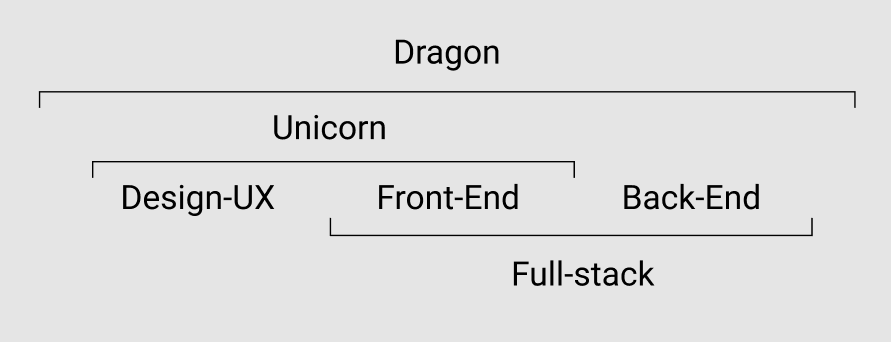
\includegraphics[scale=0.35]{dragon.PNG}}
\caption{Дракон}
\end{figure}

Знайти програміста який може дати гарантію контролю якості
на всьому спектри цих спеціалацій побідно до того, як відшукати
дракона у східній міфології, істота надзвичайно рідкіста та потужна.

\subsection{Лямбдагарбха}

Наступний рівень -- це платформоутворюючий рівень,
який включає мову програмування, рантайм та апаратуру.
Зазвичай дорослі академічні мови створюються відразу з
рантаймом, тому назвемо цю секцію рівень університетського
професора, а секцію рантайму (ОС) та апаратура назвемо
підприємницької, оскільки ОС зазвичай продають разом
із залізом і всі, хто це намагався просувати на ринок,
можна прирівняти до бодхісатств. Останні відомі лямбдагарбхи ---
це давні автори перших Лісп машин та XEROX PARC.

\begin{figure}[!htbp]
\centerline{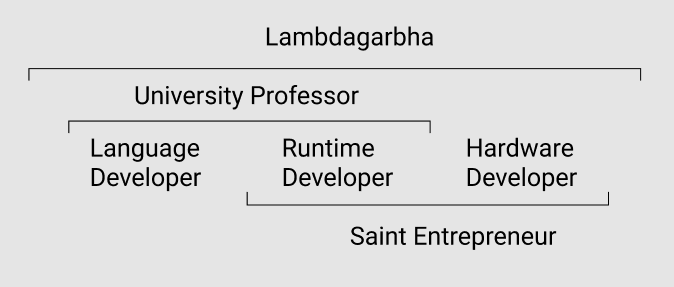
\includegraphics[scale=0.46]{lambdagarbha.PNG}}
\caption{Лямбдагарбха}
\end{figure}

Однак дракони, як майсти кінцевих продуктів, покладаються
на роботу інших потужніх божеств --- які можуть побудувати
самостійно і довести до впровадження віртуальні машини та
мови програмування, таких істот ще менше ніж драконів на платені Земля.

\newpage
\subsection{Гротендік}

На абсолютному рівні програмісти (у тому числі і топові) є
математиками, тому тут можна відзначити ядро, яке було відкрито
Квілен — модельні категорії, в яких працювали не тільки
медалісти Філдса - Воєводський і сам Квіллен, але які є
також основним інструментом сучасних теоретико-типових математиків
як Шульман. Предмет вивчає модельні категорії Квіллен назвав
гомотопічною алгеброю, за допомогою якої була побудована не
тільки модель топології алгебри самим Квілленом, але і A$^1$-теорія
гомотопій Воєводського. Усе це кришується Гротендиком, як
мультидисциплінарним програмістом абсолютного рівня (топ-математиком).

\begin{figure}[!htbp]
\centerline{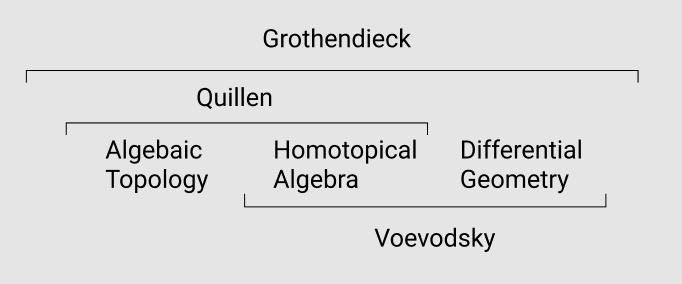
\includegraphics[scale=0.46]{grothendieck.PNG}}
\caption{Гротендік}
\end{figure}

\newpage
\subsection{Будда}

Без зайвої скромності, будь-який програміст, який зміг
не тільки уявити, а й встигнути попрацювати за життя
на всіх рівнях, може вважати себе Буддою програмування,
або як ми скромно називаємо таких пацанів — хуй з гори.

\begin{figure}[!htbp]
\centerline{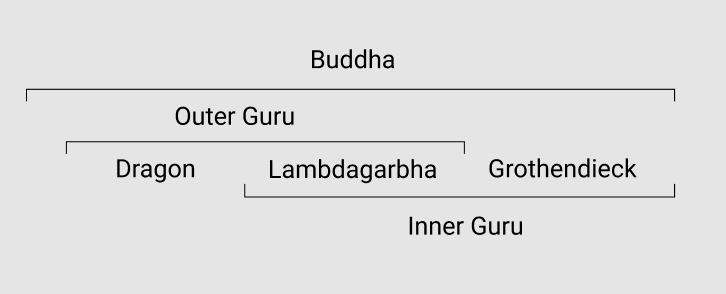
\includegraphics[scale=0.46]{buddha.PNG}}
\caption{Будда}
\end{figure}

\normalsize
